\tikzstyle{startstop} = [rectangle, rounded corners, minimum width=3.5cm, minimum height=1cm, text centered, draw=black, fill=gray!20]
\tikzstyle{process} = [rectangle, minimum width=3.5cm, minimum height=1cm, text centered, draw=black, fill=blue!10]
\tikzstyle{arrow} = [thick,->,>=stealth]

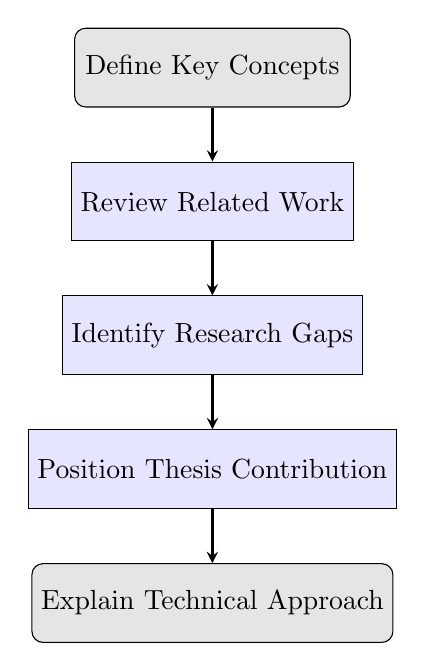
\begin{tikzpicture}[node distance=1.7cm]

\node (start) [startstop] {Define Key Concepts};
\node (review) [process, below of=start] {Review Related Work};
\node (gaps) [process, below of=review] {Identify Research Gaps};
\node (position) [process, below of=gaps] {Position Thesis Contribution};
\node (tech) [startstop, below of=position] {Explain Technical Approach};

\draw [arrow] (start) -- (review);
\draw [arrow] (review) -- (gaps);
\draw [arrow] (gaps) -- (position);
\draw [arrow] (position) -- (tech);

\end{tikzpicture}
